%% 
%% File:    PRES2024-Projet15-Fourmaux-Protocolesetperformanceduweb-RapInter.tex
%% Authors:  
%% Nils Barrellon (nils.barrellon1@etu.sorbonne-universite.fr)
%% Elyas Benyahia (Elyas.Benyahia@etu.sorbonne-universite.fr)
%% Sanjar Varatharajah (Sanjar.Varatharajah@etu.sorbonne-universite.fr)          
%% Hamza Oulfid (Hamza.Oulfid@etu.sorbonne-universite.fr)


%%%%%%%%%%%%%%%%%%%%%%%%%%%%%%%%%%%%%%%%%%%%%%%%%%%%%%%%%%%
%% Type et package

\documentclass[a4paper,12pt]{article}

\usepackage[french,english]{babel}
\usepackage{fancyhdr}
\usepackage[utf8]{inputenc}
\usepackage{cmbright}
\usepackage{epsfig}
\usepackage{calc}
\usepackage{url}
\usepackage{boxedminipage}
\usepackage{graphicx}
\usepackage[T1]{fontenc} 
\usepackage{csquotes}         % Gère les guillemets
\usepackage[backend=biber,style=numeric]{biblatex} % Pour la bibliographie


\addbibresource{PROJETRES.bib}


%%%%%%%%%%%%%%%%%%%%%%%%%%%%%%%%%%%%%%%%%%%%%%%%%%%%%%%%%%%
%%%%%%%%%%%%%%%%%%%%%%%%%%%%%%%%%%%%%%%%%%%%%%%%%%%%%%%%%%%
%% Définitions à personnaliser 

%% Pour les noms, utilisez la première lettre du prénom suivi du 
%% nom de famille (première lettre majuscule, reste en minuscule).


%%%% Indiquer le nom de l'encadrant ci-dessous:

\def\nomEncad{Olivier\_Fourmaux}

%% Si le projet est co-encadré indiquer les deux noms à la suite dans 
%% Le même champs


%%%% Indiquer les noms des étudiants participant ci-dessous:

\def\nomEtudA{Nils\_Barrellon}
\def\nomEtudB{Ilyas\_Benyahia}
\def\nomEtudC{Sanjai\_Varatharajah}
\def\nomEtudD{Hamza\_Oulfid}


%% Si le projet est encadré par moins de 4 étudiants laissez
%% les variables inutiles vides


%%%% Indiquer la référence (numero) et le nom du sujet ci-dessous:

\def\refProjet{15} 
\def\titreProjetCourt{Protocoles et perf. du web}
\def\titreProjetLong{Protocoles et performance du web}

%% Le titre court ne doit pas faire plus d'une vingtaine de caractère
%% résumez le à quelques mots essenciels


%%%% Indiquer le type de document et sa version ci-dessous:

\def\typeDoc{Rapport intermédaire}
 
%% - Rapport intermédaire






%%%%%%%%%%%%%%%%%%%%%%%%%%%%%%%%%%%%%%%%%%%%%%%%%%%%%%%%%%%
%%%%%%%%%%%%%%%%%%%%%%%%%%%%%%%%%%%%%%%%%%%%%%%%%%%%%%%%%%%
%% Définitions à ne pas modifier
 
%%%%% ||| Mise en page verticale ||| 
\setlength{\voffset}{-1in} % a4:reste 297mm pour les 5 suivants:
\setlength{\topmargin}{15mm}         % avant l'en-tête
\setlength{\headheight}{20mm}        % hauteur de l'en-tête 
\setlength{\headsep}{10mm}            % entre l'en-tête et le corps
\setlength{\textheight}{220mm}       % hauteur du corps
\setlength{\footskip}{12mm}          % pied de page par rapport au corps 

%%%%% --- Mise en page horizontale ---
\setlength{\hoffset}{-1in} % a4:reste 210mm 
\setlength{\oddsidemargin}{25mm}     % entre hoffset et le corps
\setlength{\evensidemargin}{25mm}    % entre hoffset et le corps
\setlength{\marginparwidth}{0mm}     % largeur de la marge
\setlength{\marginparsep}{0mm}       % séparateur corps marge
\setlength{\textwidth}{160mm}        % largeur du corps

\def\annee{2024-25}

\renewcommand{\familydefault}{\sfdefault}


%%%%%%%%%%%%%%%%%%%%%%%%%%%%%%%%%%%%%%%%%%%%%%%%%%%%%%%%%%%
%% Début du document

\begin{document}
%\sffamily
\selectlanguage{french}



%%%%%%%%%%%%%%%%%%%%%%%%%%%%%%%%%%%%%%%%%%%%%%%%%%%%%%%%%%%
%% Définition des en-têtes et pied de pages
\pagestyle{fancyplain}
\lhead[\fancyplain{}{Master Informatique\\ UE \textbf{PRes} fév. \annee \\ \nomEncad}]
      {\fancyplain{}{Master Informatique\\ UE \textbf{PRes} \annee \\ \nomEncad}}
\chead[\fancyplain{}{\textbf{Projet \refProjet\\\titreProjetCourt}}]
      {\fancyplain{}{\textbf{Projet \refProjet\\\titreProjetCourt}}}
\rhead[\fancyplain{}{\nomEtudA\\\nomEtudB\\\nomEtudC\\\nomEtudD}]
      {\fancyplain{}{\nomEtudA\\\nomEtudB\\\nomEtudC\\\nomEtudD}}
\lfoot[\fancyplain{}{
\includegraphics[width=3cm]{LOGO_SCIENCES_DEF_CMJN_med.jpg}}]
      {\fancyplain{}{
\includegraphics[width=3cm]{LOGO_SCIENCES_DEF_CMJN_med.jpg}}}
\cfoot[\fancyplain{}{\textbf{\thepage/\pageref{fin}}}]
      {\fancyplain{}{\textbf{\thepage/\pageref{fin}}}}
\rfoot[\fancyplain{}{\typeDoc}]
      {\fancyplain{}{\typeDoc}}

%%%%%%%%%%%%%%%%%%%%%%%%%%%%%%%%%%%%%%%%%%%%%%%%%%%%%%%%%%%

~

      \begin{center}
        \begin{boxedminipage}{12cm}{
            \begin{center}
              ~\\\LARGE\textbf{\titreProjetLong}\\
              ~\\\large Encadrant: \textbf{\nomEncad,}\\
              ~\\\large Etudiants: \textbf{\nomEtudA, \nomEtudB, \nomEtudC, \nomEtudD}\\
              ~
            \end{center}
            }
        \end{boxedminipage}
      \end{center}

~

\tableofcontents

\newpage

\section{Cahier des charges}


\subsection{Description générale}
Les protocoles pour acceder au web ont évolué à différents niveaux : IPv4 ou IPv6, TCP ou UDP-QUIC, et HTTP1.1 ou HTTP2 ou HTTP3. Les trafics sont souvent chiffrés, particulièrement avec QUIC/HTTP3, ce qui rend plus complexe leurs études, mais pas impossible grâce aux capacités des analyseurs à utiliser les clés privées que certains clients peuvent leur fournir. Le but de ce projet est de découvrir les protocoles utilisées par les principaux sites, d'en déchiffrer les paramétrages et d'en évaluer la performance.

\subsection{Travail à réaliser}
Plusieurs travaux aux dates limite échelonnées sont à réaliser :
\begin{itemize}
\item Analyse des différentes normes autour du protocole HTTP : recherche bibliographique et étude puis synthèse des documents trouvés,
\item Etude des outils/librairies disponibles pour générer du trafic HTTP1.1, HTTP2, HTTP3 en récupérant les clés privées et en déchiffrant la partie contrôle du trafic,
\item Réalisation d'un outil crawler qui parcours les sites du top 1000 afin de caractériser le paramétrage de chacun d'entre eux, de fournir des statistiques d'usage et de performance. Pour les mesures de performance, les même sites accessibles via les différentes versions de HTTP seront recherchés et comparés.
\end{itemize}
Ces différents travaux vont nécessiter l'acquisition de nouvelles compétences, notamment :
\begin{itemize}
\item découverte et utilisation de l'interface en ligne \textbf{Curl} ;
\item apprentissage du logiciel \textbf{Zotero} pour la création d'une bibliographie correctement normée ;
\item apprentissage de la recherche en ligne et en bibliothèque (à l'aide des tutoriels proposés par la BU).
\end{itemize}





\section{Plan de développement}
\subsection{Diagramme de Gantt}
Ci-dessous le diagramme de Gantt établi à la naissance du projet (début novembre).
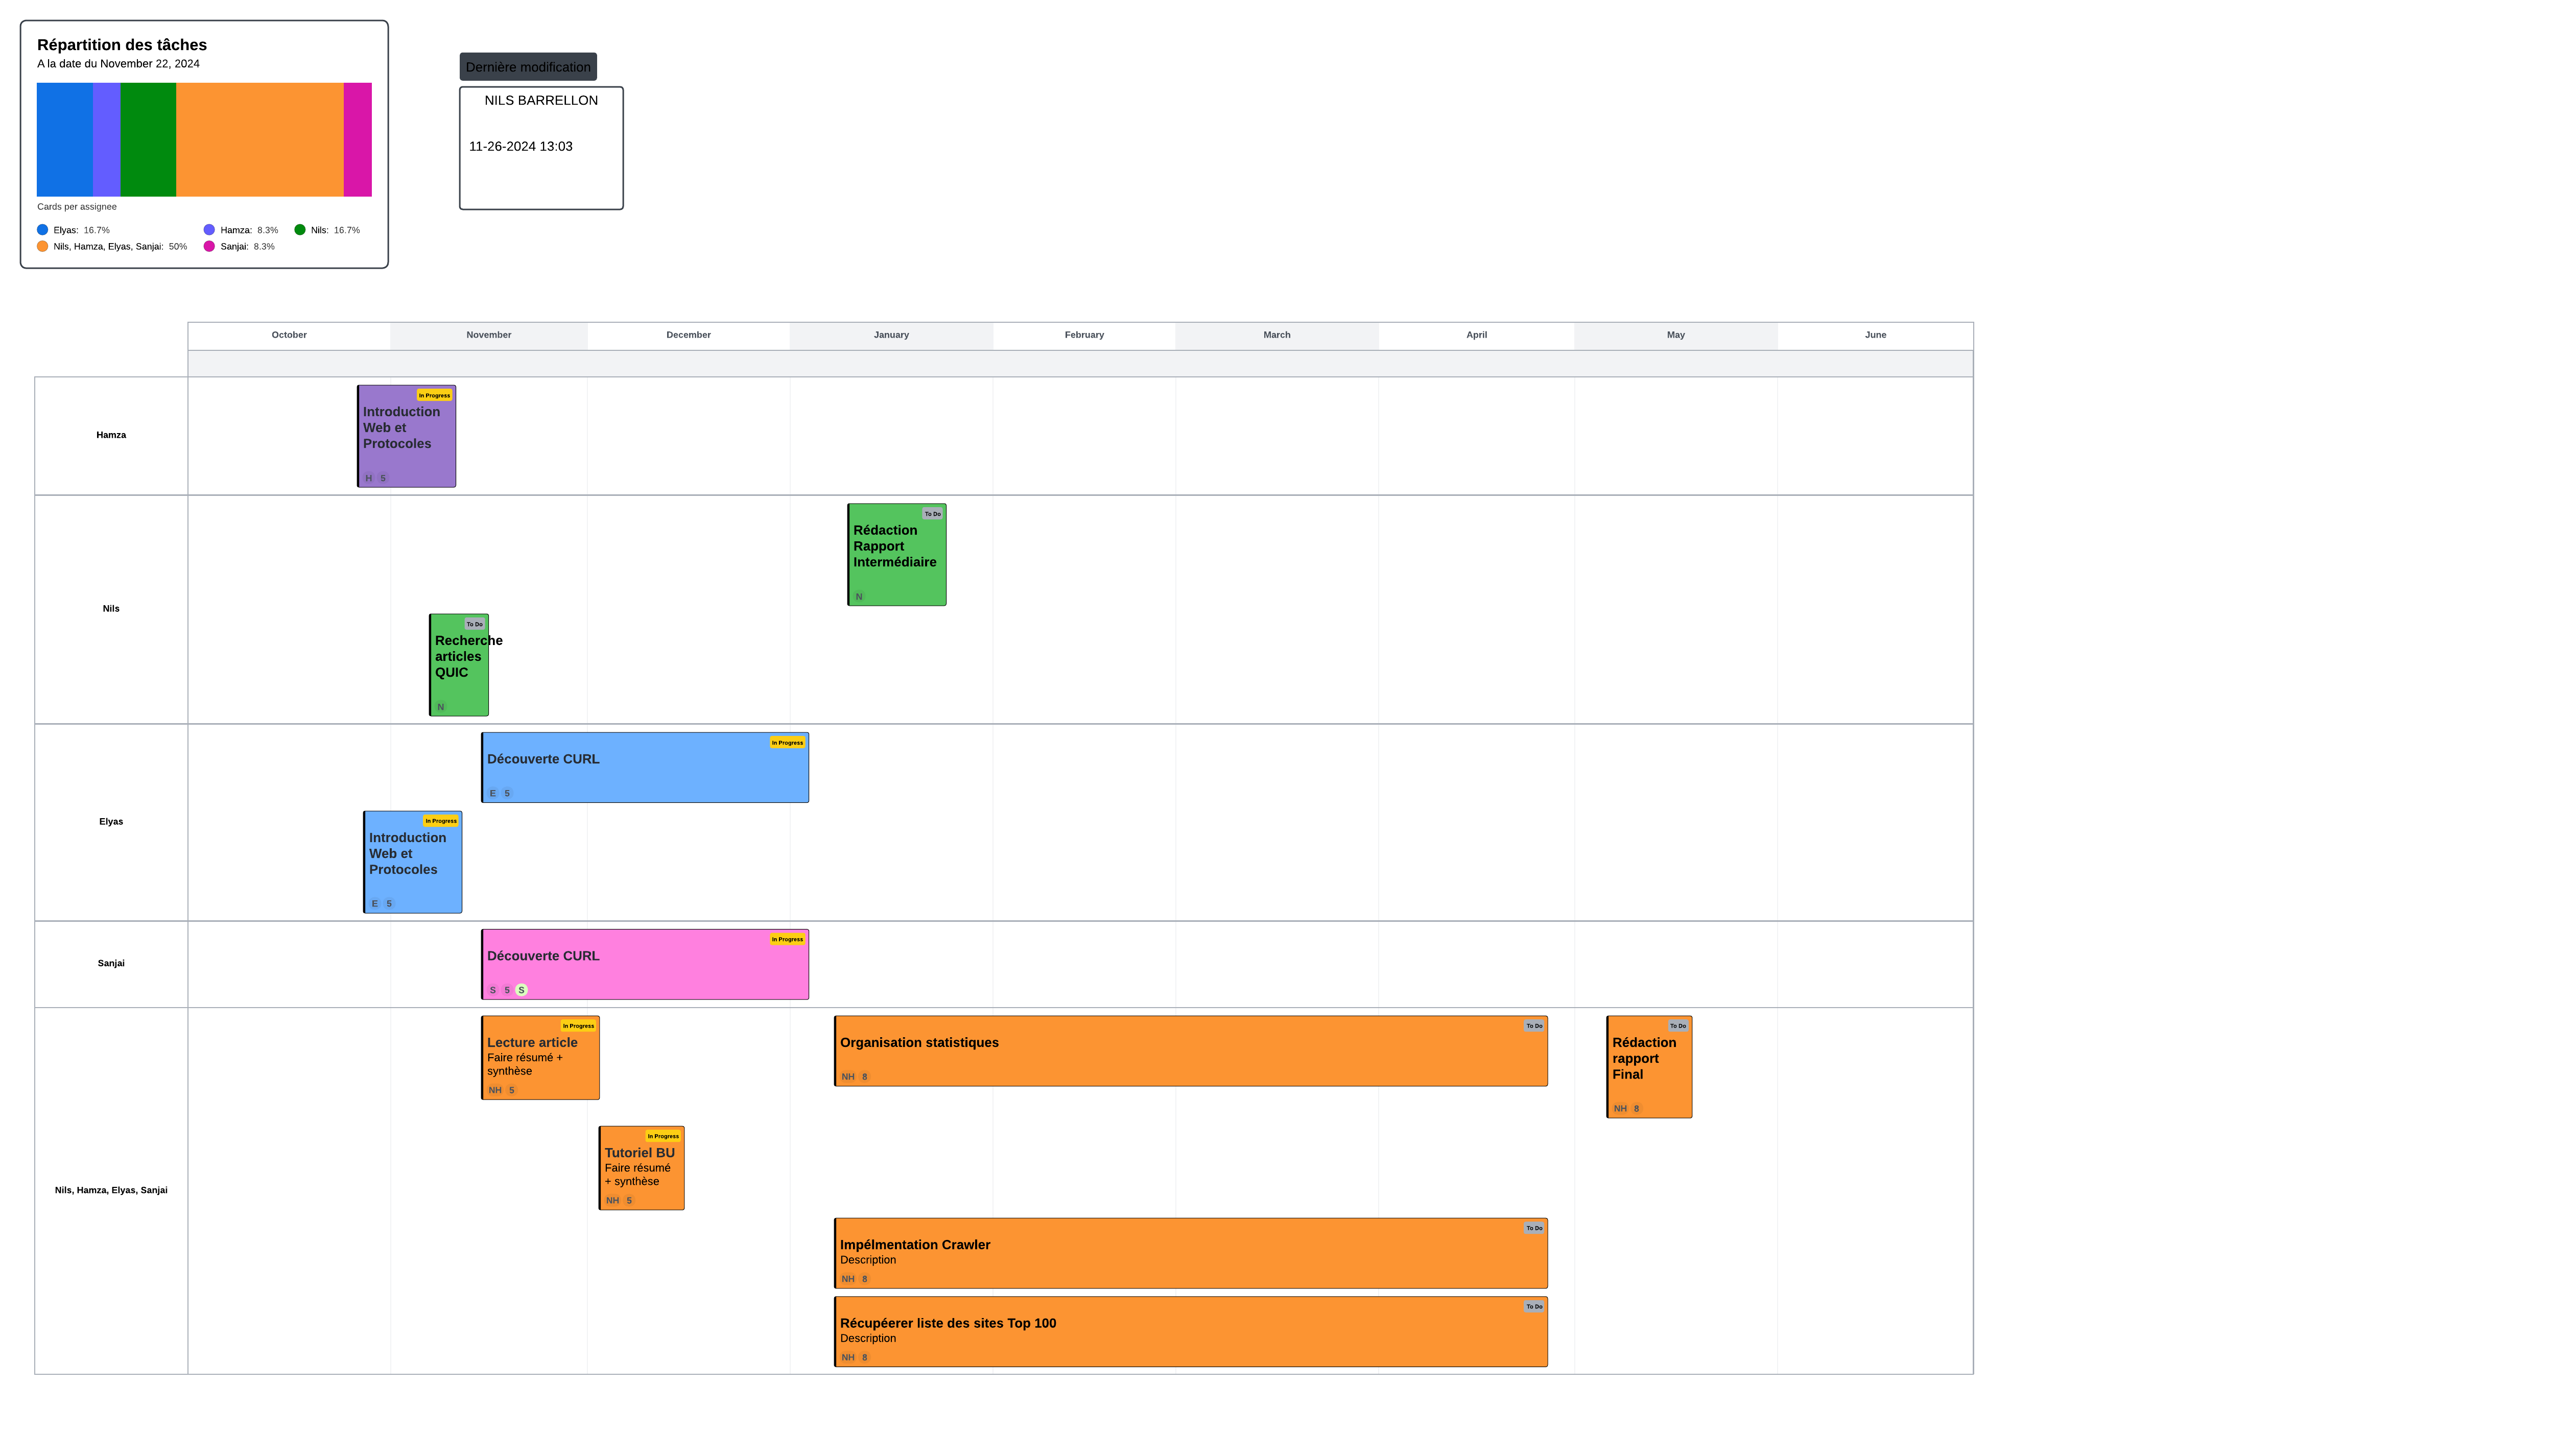
\includegraphics[width=15cm]{Gantt chart.png}

\subsection{Fait. A faire}
Il nous a semblé judicieux de commencer par une recherche bilbiographique sur le protocole QUIC que nous n'avons pas étudié en cours. Après quelques articles et videos de vulgarisation \cite{Capitole_du_Libre_2019} Le site de recherche de la librairie de l'Association for Computing Machinery nous a permis de trouver une dizaine d'articles concernant le protocole QUIC et ses performances, notamment en comparaison de celles offertes par le protocole TCP. Nous nous sommes répartis la lecture de ces articles, leur résumé et leur synthèse. Dans le même temps, la moitié du groupe s'est lancée dans la découverte de Curl dont nous aurons besoin pour la réalisation du crawler (dont la conception est pour l'instant programmée au deuxième semestre).

Parallèlement, nous avons suivi la formation proposée par la bibliothèque pour l'utilisation de Zotero notamment qui permet l'établissement d'une bibliographie conforme aux normes en vigueur. Nous avons choisi celle de l'IEEF. 

\section{Bibliographie}

\printbibliography

\section{Analyse}

\subsection{Introduction}
Le World Wide Web, plus communément appelé le web, est un système révolutionnaire de
documents hypertexte, interconnectés et accessibles via Internet. Il a transformé l'accès,
le partage et la diffusion de l'information à l'échelle mondiale.

Le développement du World Wide Web remonte au début des années 1990, lorsque le
scientifique britannique Tim Berners-Lee, travaillant au CERN (Organisation Européenne
pour la Recherche Nucléaire), a proposé l'idée d'un système d'information distribué. En
1991, Berners-Lee a présenté le premier navigateur web et serveur web, offrant une
interface conviviale pour accéder et naviguer dans les documents hypertexte sur Internet.
Au cœur du World Wide Web se trouve le protocole de transfert hypertexte (HTTP), qui
facilite le transfert de documents hypertexte entre serveurs web et navigateurs. HTTP
permet aux utilisateurs de demander et de récupérer des pages web depuis des serveurs
distants, rendant possible une navigation fluide entre des documents interconnectés via
des hyperliens.

La structure décentralisée et interconnectée du web, basée sur l'hypertexte, encourage un
écosystème où les utilisateurs peuvent explorer divers sujets et découvrir de nouvelles
sources de connaissance. Cette approche non linéaire marque une rupture avec les
médias imprimés traditionnels, où la navigation et l'exploration sont limitées.
Avec l'arrivée de navigateurs graphiques tels que Mosaic et Netscape Navigator dans les
années 1990, le World Wide Web s'est popularisé, devenant accessible à un large public
et entraînant une croissance exponentielle de l'usage d'Internet. Ces navigateurs ont
intégré des fonctionnalités telles que les favoris, l'historique et les capacités de recherche,
améliorant considérablement l'expérience utilisateur.
\subsection{Les protocoles HTTP}
Depuis sa création, le protocole HTTP a évolué pour répondre aux besoins croissants en
termes de performances, de sécurité et de scalabilité.
\begin{itemize}
\item
La première version, HTTP/0.9, introduite en 1991, était rudimentaire et permettait
seulement de récupérer des pages HTML en texte brut, sans support pour les en-têtes ou
des fonctionnalités avancées. En 1996, HTTP/1.0 a apporté une amélioration majeure
avec l'introduction des en-têtes HTTP, permettant la gestion des métadonnées et des
contenus variés tels que les images et vidéos.  
\item
En 1997, HTTP/1.1 a marqué une étape clé
avec des fonctionnalités comme la connexion persistante, qui réutilise la même connexion
TCP pour plusieurs requêtes, la prise en charge des requêtes partielles pour les fichiers
volumineux, et une meilleure gestion des proxys et caches.
\item

HTTP/2, introduit en 2015, a
été conçu pour améliorer les performances en intégrant des fonctionnalités telles que la
multiplexation des requêtes sur une seule connexion, la compression des en-têtes pour
réduire la surcharge réseau et le support natif du chiffrement via TLS (bien que non
obligatoire). 
\item

Enfin, HTTP/3, basé sur le protocole QUIC et apparu en 2018, a introduit des
avancées significatives en utilisant UDP au lieu de TCP, réduisant ainsi la latence, offrant
une meilleure gestion des pertes de paquets et rendant les connexions plus robustes. De
plus, HTTP/3 impose un chiffrement obligatoire, renforçant la sécurité des
communications.
\end{itemize}
Les normes entourant HTTP, définies par l'IETF (Internet Engineering Task Force),
garantissent son interopérabilité et son évolution. Ces normes incluent des RFC détaillant
les différentes versions du protocole et leurs extensions associées, assurant ainsi leur
mise en œuvre cohérente et efficace à travers le monde.
\subsection{Les protocoles de transport}
\subsubsection {Le protocole TCP}

Le protocole TCP voit le jour dans les années 70. Protocole fiable, encapsulé dans un paquet IP, il assure une connexion de bout en bout. A ce jour, il est LE\footnote{La finalité de ce travail est de le confirmer ou de l'infirmer} protocole de transport sur Internet. Il a connu de nombreuses améliorations au fil des décennies, en témoignent les Request For Comments{ajouter Référence vers dernier RFC TCP} nombreuses, la première étant numérotée 761, la dernière 9293\cite{eddy_transmission_2022}.

L'établissement d'une connexion TCP, par exemple pour l'obtention d'une page web nécessite le 3-Way HandShake où trois segments SYN, SYN-ACK et ACK sont échangés avant de pouvoir échanger des données.


\begin{figure}
    \centering
    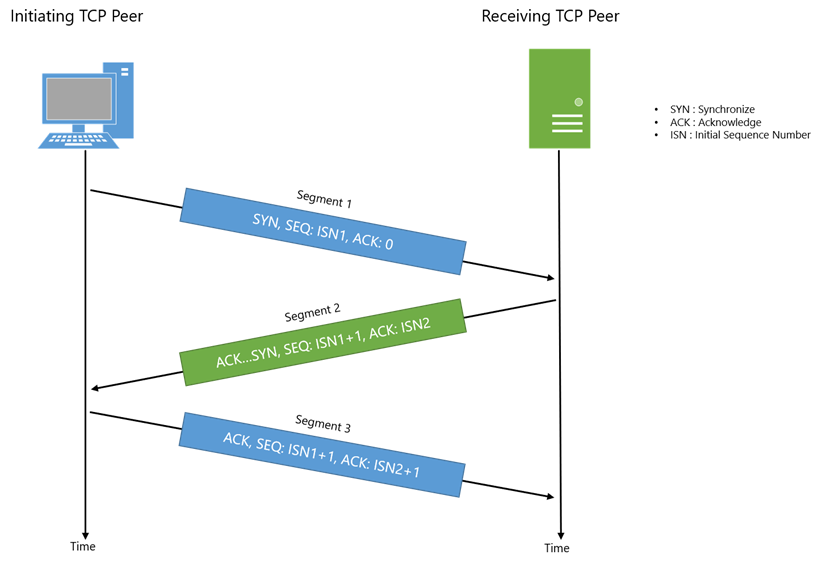
\includegraphics[width=0.5\linewidth]{120818_0035_TheTCP3Wayh1.png}
    \caption{Protocole TCP. Etablissement de la connexion par 3-Way Handshake}
    \label{fig:3-Way Handshake}
\end{figure}

La figure 1 \footnote{https://www.johnpfernandes.com/2018/12/08/the-tcp-3-way-handshake/} montre ainsi que l'établissement de cette connexion a une durée incompressible due au Round Trip Time entre le client et le serveur. Des options comme FastTCP permettant de faire une requête GET simultanément au paquet de synchronisation ont été introduites il y a quelques années mais n'ont jamais résolues le problème car il n'est pas reconnu par les middleboxes qui le bloquent.
Par la suite, le besoin de sécurité a imposé de crypter les données contenues dans les segments échangés. Cela a été fait par l'ajout de la couche TLS allongeant les délais de connexion, car au moins deux tours sont nécessaires à son établissement (2-RTT)  comme le montre la Figure 2\footnote{https://www.cloudflare.com/fr-fr/learning/ssl/what-happens-in-a-tls-handshake/}.

\begin{figure}
    \centering
    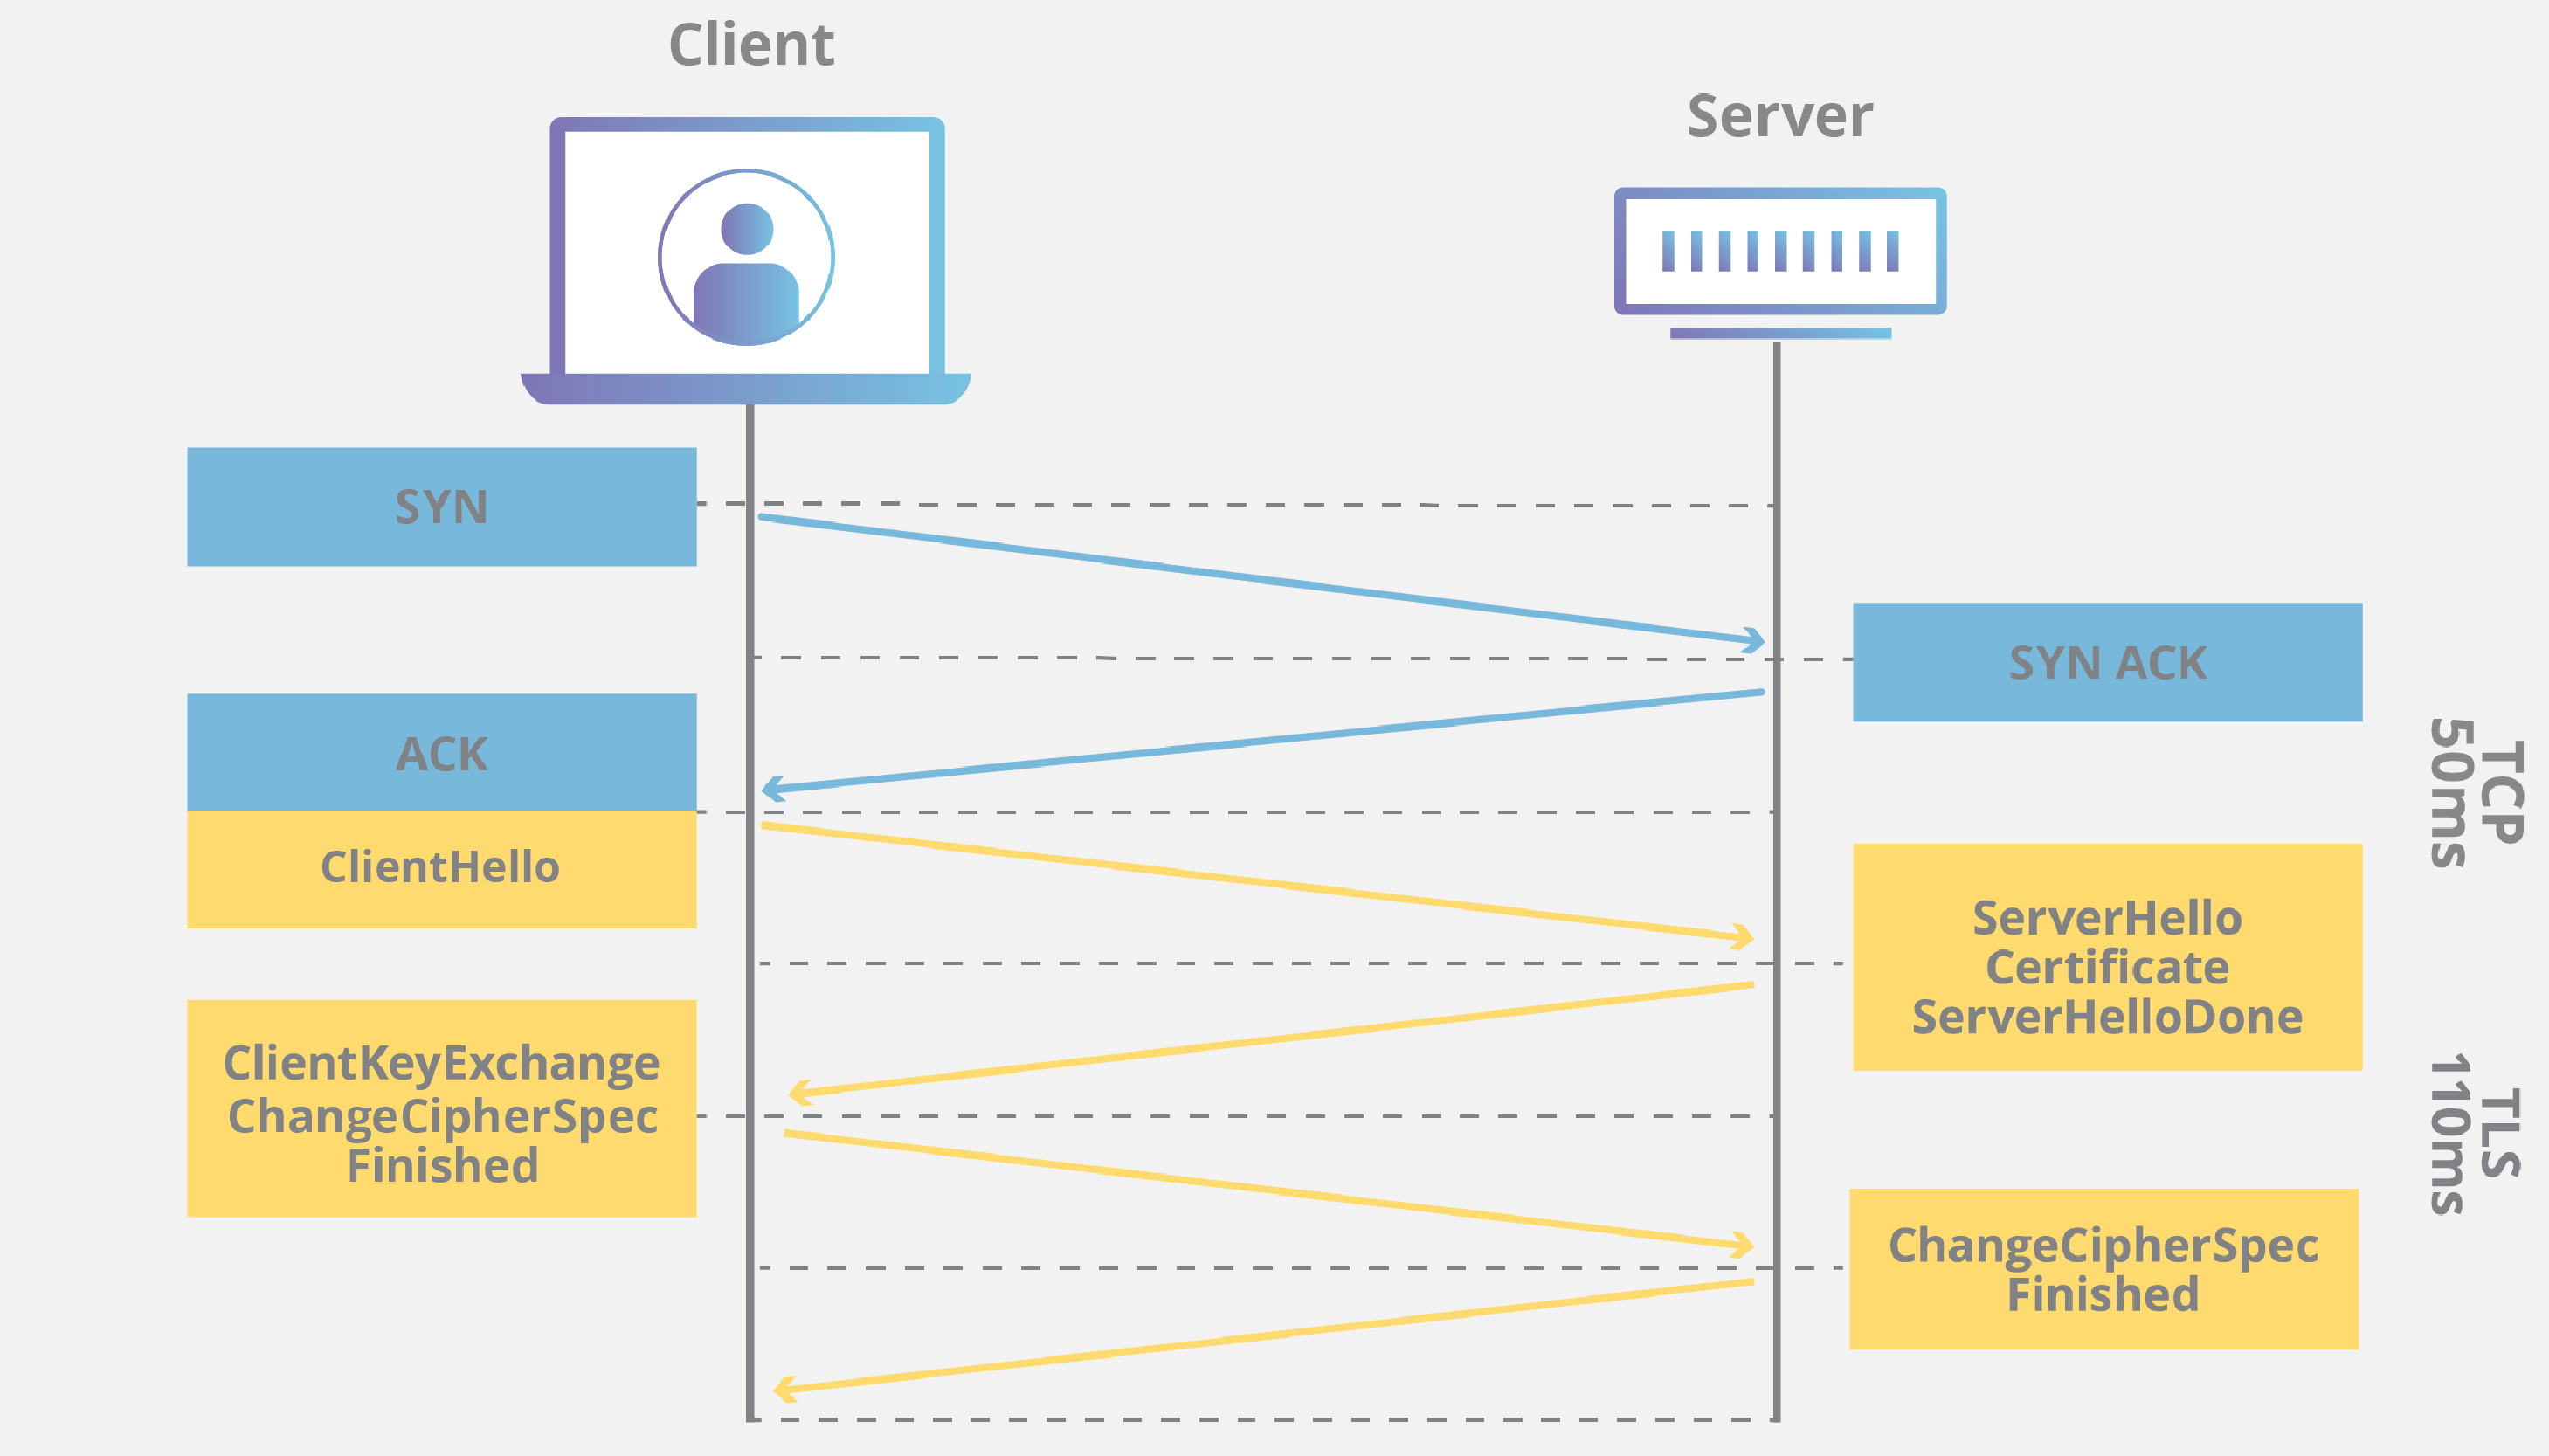
\includegraphics[width=0.5\linewidth]{tls-ssl-handshake.png}
    \caption{Protocole TCP avec la couche TLS. Etablissement de la connexion.}
    \label{fig:`tls-ssl-handshake' }
\end{figure}

L'utilisation massive du protocole TCP et son implémentation dans le noyau du système, qui complique grandement les modifications que pourraient apporter la communauté, expliquent son adoption unanime malgré ses problèmes de latence. Ce phénomène met en évidence l'ossification de l'Internet : implémenter un nouveau protocole est très difficile à réaliser...

Néanmoins, dans les années 2010, Google va se lancer dans cette expérimentation car, de nombreux utilisateurs ont adopté le navigateur qu'il a développé (Chrome) pour faire des requêtes sur ses serveurs. L'entreprise étant donc aux deux bouts de la chaine de transport, elle peut implémenter un nouveau protocole de transport appelé QUIC et encapsulé dans UDP. Le HTTP/3 était né : soit la combinaison du protocole HTTP, transporté par QUIC. Il est à noter que, depuis, QUIC est devenu un protocole de transport qui n'est pas uniquement dédié à HTTP, ni aux requêtes de Chrome en direction des serveurs de Google.

\subsubsection {Le protocole QUIC}

Le protocole QUIC est décrit dans les RFC 8999,9000,9001 et 9002\cite{iyengar_quic_2021}. 


Étant donné que UDP n’est pas fiable, QUIC implémente les retransmissions et contrôle
de congestion dans la couche application.

Ce protocole offre un multiplexage amélioré, il permet d'envoyer plusieurs requêtes
simultanément sur une seule connexion UDP, éliminant les blocages liés à l'ordre des
paquets.

Contrairement à HTTP/1.1 qui nécessite plusieurs RTT pour l'établissement d'une
connexion sécurisée, QUIC peut réduire la latence à un seul RTT ou même zéro RTT si le
client et le serveur ont déjà échangé auparavant.

QUIC gère aussi son propre algorithme de chiffrement (auparavant géré par TLS) nommé
QUIC-Crypto et intègre un module de Correction d'Erreur Avancée (Forward Error
Correction, inactif par défaut) pour compenser les pertes dans un groupe de paquets sans
devoir retransmettre systématiquement.

QUIC utilise des algorithmes de contrôle de congestion comme CUBIC TCP, mais avec
des ajustements spécifiques pour mieux gérer les pertes et maximiser l'utilisation du
réseau. Contrairement à TCP, où les connexions sont liées aux adresses IP et aux ports,
QUIC utilise un identifiant de connexion unique CID (au niveau de la couche application),
facilitant la gestion des changements d'adresses IP, par exemple dans les réseaux
mobiles.

\subsection{TCP vs QUIC}

L'étude de Fan Liu et Patrick Crowley\cite{liu_security_2023} examine les
performances de QUIC et HTTP/3 en termes de rapidité, de fiabilité et de gestion des
connexions, en les comparant à TCP et HTTP/2. 

L’étude s’appuie sur des tests en environnements contrôlés pour évaluer les
performances sous différentes conditions réseau. Les ressources testées incluent des
fichiers statiques de tailles variées, allant de 0 octet à 10 Mo, ainsi que des pages web
réelles provenant de Google, Facebook et Cloudflare, classées par taille (petites,
moyennes et grandes). Les serveurs de test utilisent Nginx-quic, tandis que les clients
incluent des navigateurs et outils compatibles avec HTTP/2 et HTTP/3, comme
Chromium, Curl et Proxygen. Les conditions réseau simulées comportent quatre
scénarios : une connexion sans délai ni perte de paquets, une perte de paquets de 5 %,
un délai de 200 ms sans perte, et une combinaison des deux derniers cas. Les
performances sont mesurées par le temps jusqu’au dernier octet (TTLB) pour les
fichiers simples et l’indice de vitesse (SI) pour les pages web.

Les résultats montrent que QUIC et TCP ont des performances comparables lorsque le
réseau est stable, sans délai ni perte. Cependant, lorsque le délai atteint 200 ms, QUIC
devient supérieur pour les fichiers inférieurs à 100 Ko, car son handshake rapide réduit
l’impact de la latence. Pour les fichiers plus volumineux, cette différence s’atténue. En
présence de pertes de paquets, QUIC reste compétitif en ajustant son débit de manière
proactive grâce à ses signaux de congestion explicites, contrairement à TCP qui
interprète les pertes comme des signes de congestion réseau. Lorsque des pertes de
paquets et un délai sont combinés, QUIC dépasse TCP, notamment sur les fichiers de
grande taille.

En conclusion, QUIC surpasse TCP dans des environnements dégradés, notamment en
cas de faible bande passante, de grande latence ou de perte de paquets



De nombreux autres articles montrent que le protocole QUIC est plus efficace dans la majeure partie des configurations. \cite{mucke_reacked_2024} \cite{muthuraj_replication_2024} \cite{yu_dissecting_2021} Ainsi, on peut se demander, comme s'interrogent beaucoup sur le web, si QUIC est amené à supplanter TCP sous peu.



\section{Conception}
La finalité du projet est de dresser des statistiques sur les 100 sites les plus consultés au monde : quel pourcentage utilise le protocole HTTP/3 ? Il va falloir pour cela étudier les échanges TCP avec ses serveurs. Il conviendra de décrypter les paquets QUIC. Les échanges seront faire en ligne de commande cURL et il faudra les automatiser avec un programme (en bash ? En C ? En python ?). Il faudra peut-être envisager de travailler avec plusieurs navigateurs, QUIC ayant été développé pour Chrome. Ce protocole est-il à l'oeuvre pour des requêtes effectuées depuis un autre navigateur ?
\subsection{cURL}

\subsection{Décryptage}
\subsection{Liste des 100 sites les plus visités}
\subsection{Mise en place d'un crawler}
Dans quel langage programmer les instructions cURL ?
\section{Etat d'avancement/Compte rendu}
Fin décembre 2024, l'état d'avancement est le suivant :
\begin{itemize}
\item
Nous avons mieux cerné le protocole QUIC dont nous ignorions l'existence jusqu'alors. Néanmoins, après lecture d'articles étudiant les principaux avantages de QUIC (notamment par rapport à TCP) nous n'avons pas poussé plus avant son étude et ses mécanismes. En effet, nous avons considéré que cela ne rentrait pas dans le cadre de notre projet.

\item
Nous avons étudié expérimentalement (à l'aide de captures Wireshark) les connexions du navigateur Chrome sur un serveur de Google (youtube par exemple). L'utilisation de QUIC n'est pas anecdotique.
\item
Nous avons mieux cerné le projet et ses attendus.
\item
Les tutoriels de la BU nous ont permis d'entamer la création d'une bibliographie normée à intégrer dans notre rapport. Rapport que nous avons choisi de rédiger en Latex, à l'aide de l'éditeur Tex Maker.


\end{itemize}

\section{Annexe A}

Deux captures d'écran d'une analyse de trames par WireShark lors d'un appel depuis Google Chrome à un serveur Google (youtube.fr). 

\begin{figure}
    \centering
    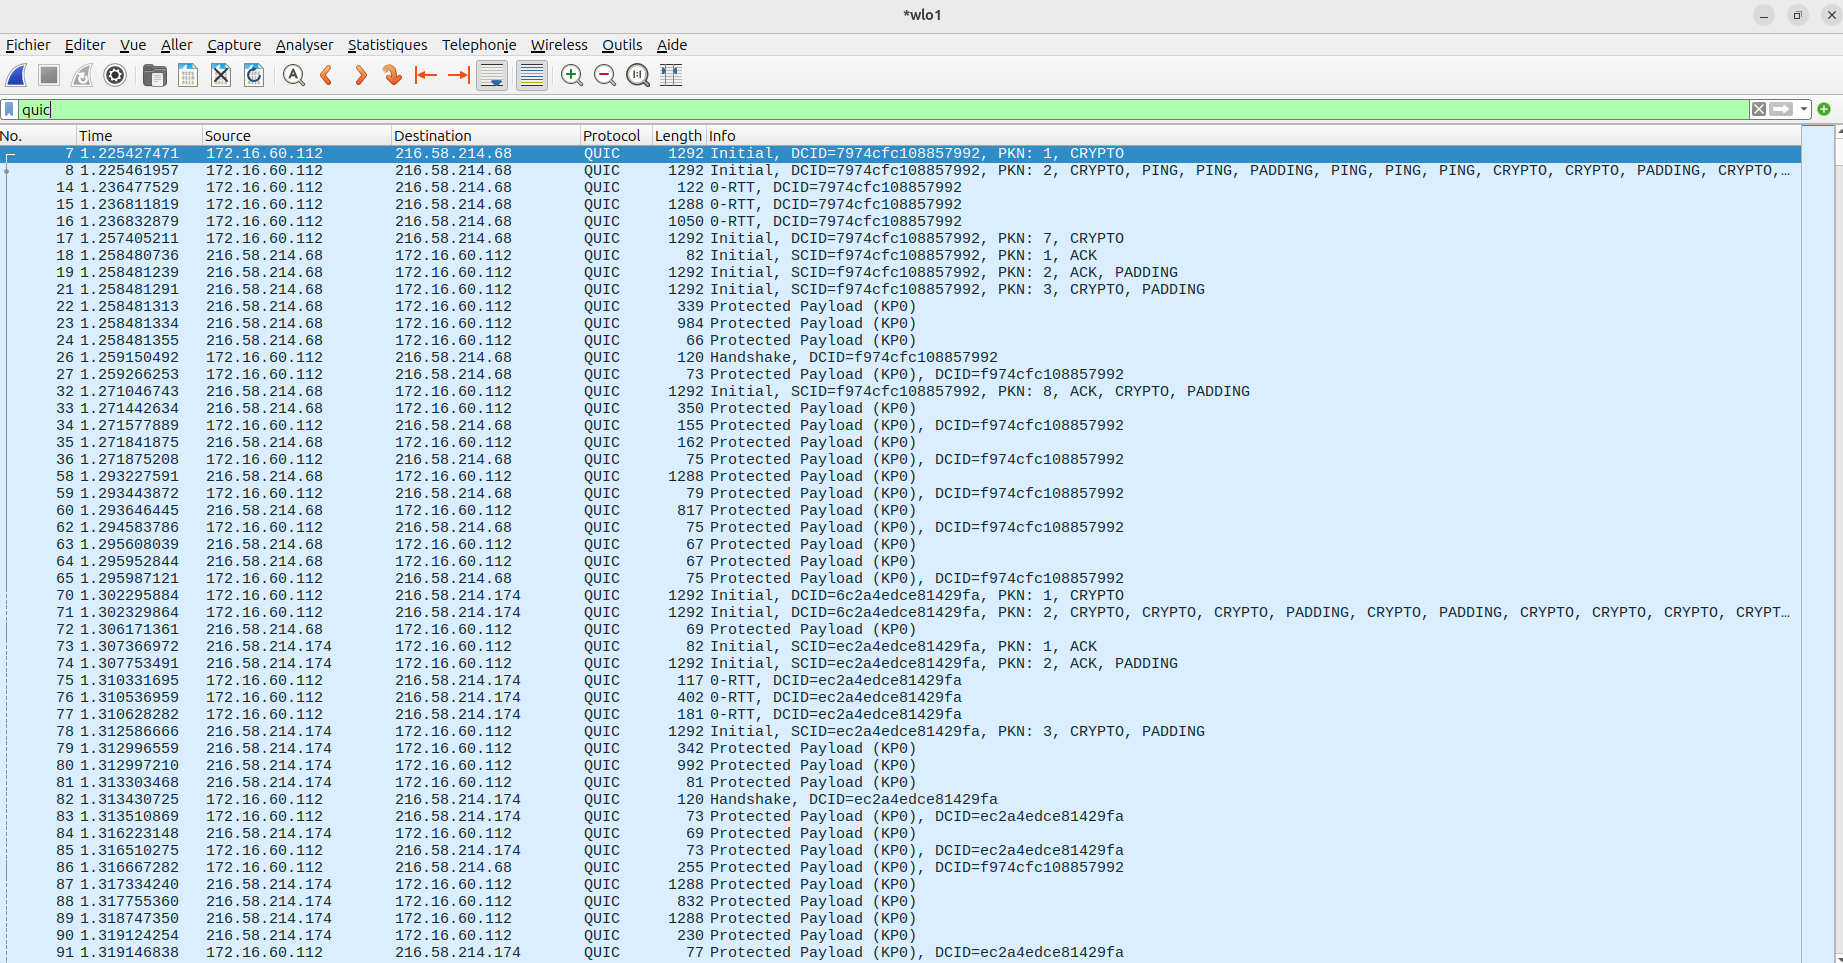
\includegraphics[width=1\linewidth]{Wire Shark QUIC.png}
    \caption{Capture WireShark. Requête depuis Google Chrome vers Youtube.fr}
    \label{fig:QUIC1}
\end{figure}

\begin{figure}
    \centering
    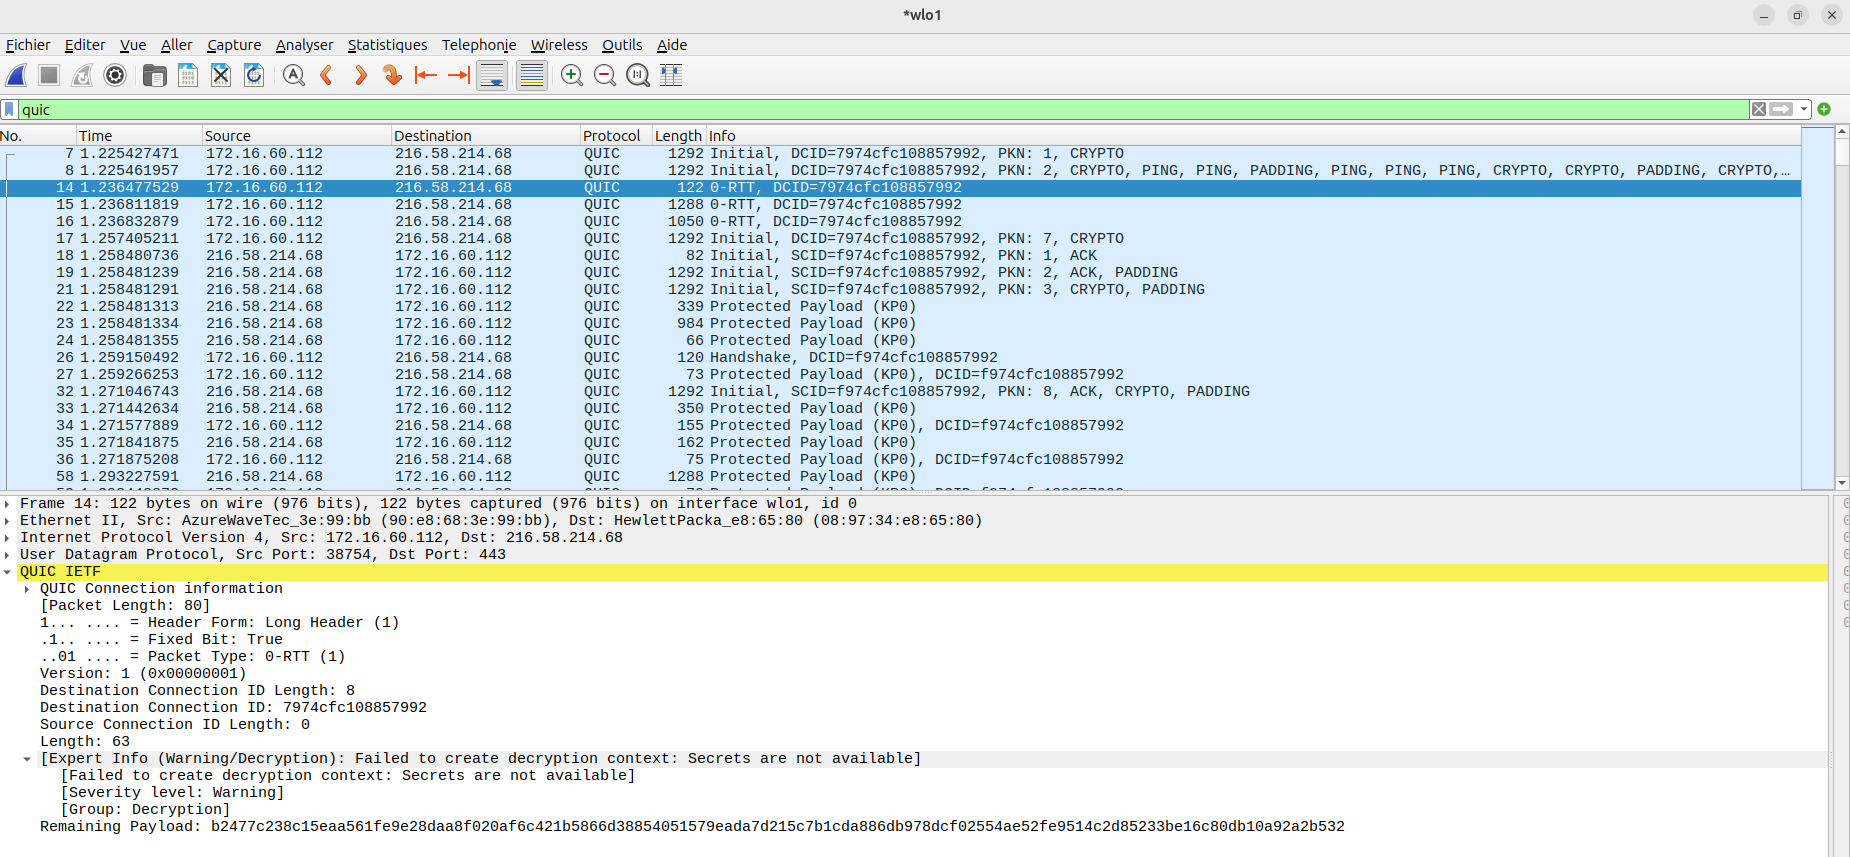
\includegraphics[width=1\linewidth]{Wire Shark Capture QUIC.png}
    \caption{Capture WireShark. Requête depuis Google Chrome vers Youtube.fr. Zoom 0-RTT}
    \label{fig:QUIC1}
\end{figure}
\label{fin}

\end{document}

